
\begin{frame}
\frametitle{Introduction to Reputation systems}
\begin{center}
\begin{tikzpicture}
  \node (img1) {
\includegraphics[height=3cm]{netflix-logo.png}};
  \node (img2) at (img1.north) [xshift = 0cm,yshift = 1cm] {
\includegraphics[height=2cm]{netflixStars.jpg}};
  \node (img3) at (img2.east) [xshift = 1.5cm,yshift = 0.5cm] {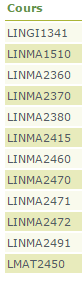
\includegraphics[height=4cm]{ucl.png}};
  \node (img4) at (img3.east) [xshift = 2cm] {
\includegraphics[width=4cm]{amazon-ratings.png}};
  \node (img5) at (img4.south) [yshift = -0.3cm] {\includegraphics[width=3cm]{Amazon.png}};
  \node (img6) at (img5.south) [xshift = 0cm,yshift = -1.2cm] {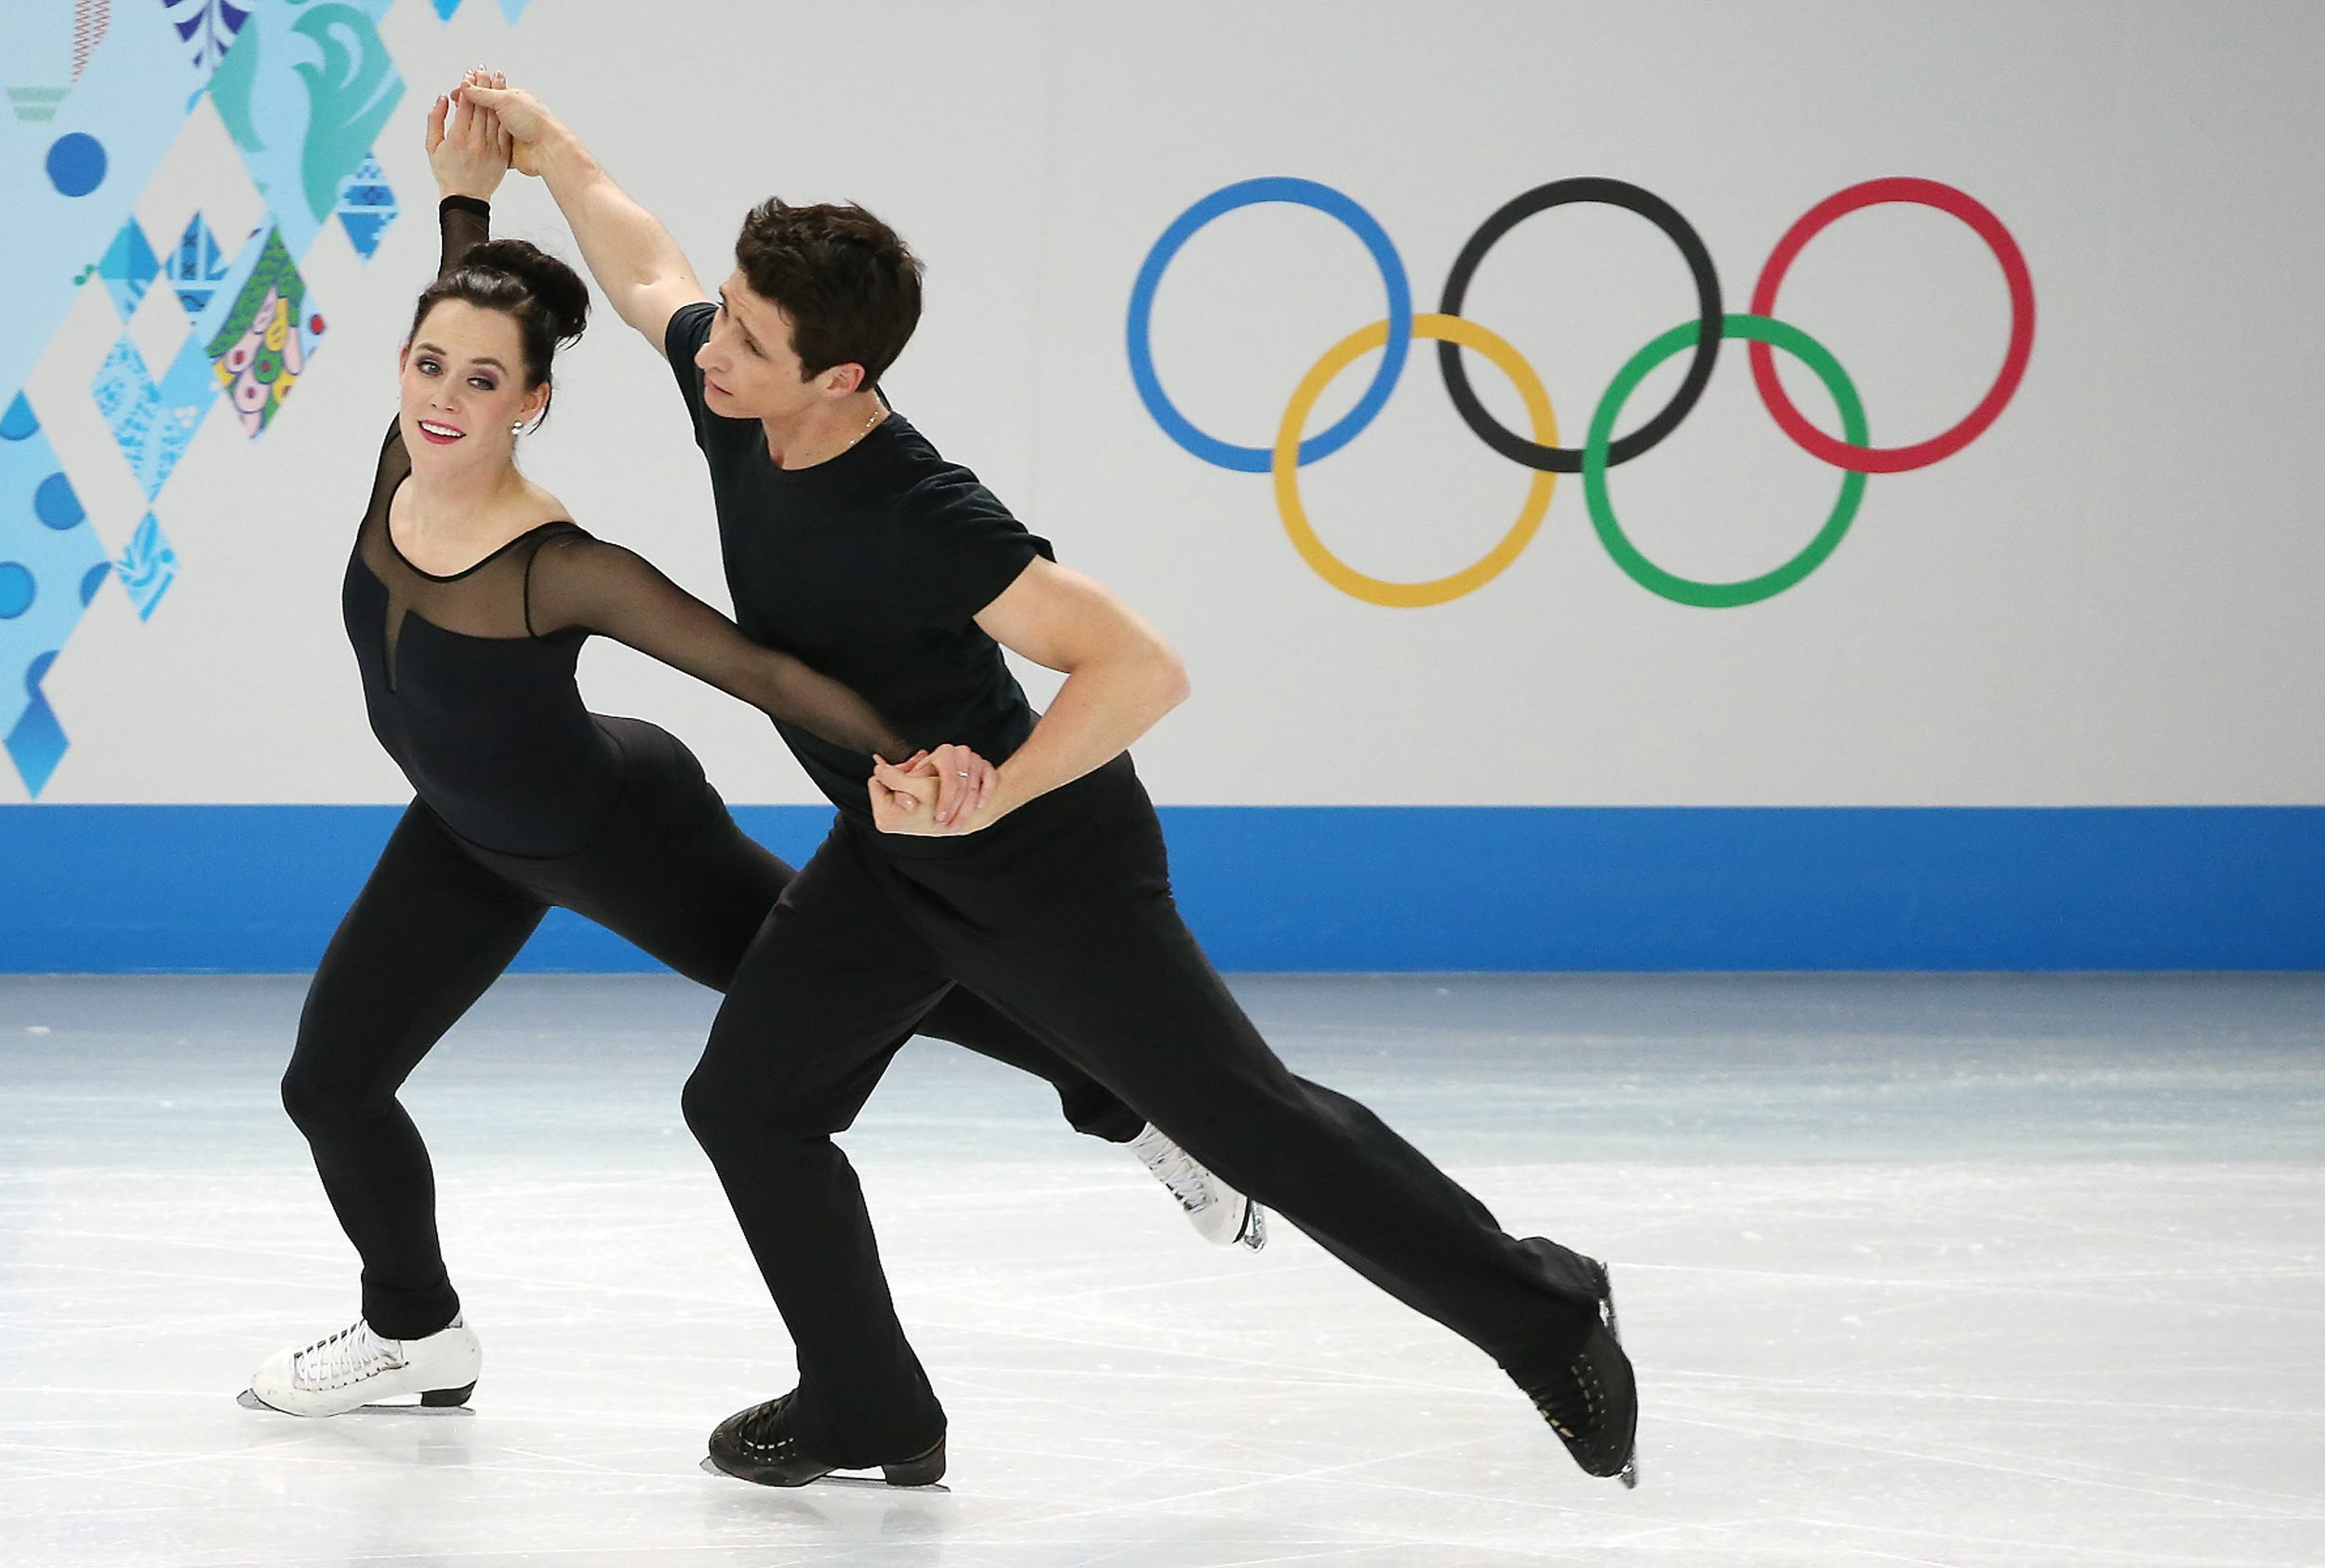
\includegraphics[width=4.5cm]{SochiOlympics.jpg}};
  \node (img7) at (img6.south west) [xshift = 0cm] {
\includegraphics[width=3cm]{tripadvisor.jpg}};
\end{tikzpicture}
\end{center}
\end{frame}

\begin{frame}[allowframebreaks]
\frametitle{Reminder}
\begin{block}{Actors}
$N$ judges, $M$ objects and $K$ characteristics
\end{block}
\begin{block}{Tensors in use}
\centering
\begin{tabular}{@{}ccl@{}}
\hline
Tensor & Size                  & Definition                                                                                                     \\ \hline
$X$    & $N \times M \times K$ & IN : $X_{ijk}$ is the evaluation given by rater i\\
          &                                     &  to object j on characteristic k. \\
$A$    & $N \times M \times K$ & IN : The adjacency matrix. $A_{ijk} = 1$ if \\
          &                                & rater $i$ evaluates $j$ on characteristic $k$, \\
          &                                & otherwise $A_{ijk} = 0$. \\
$m_i$ & $N \times 1$          & IN : Sum of characteristics evaluated by i. \\                                                        
$R$    & $M \times K$          & OUT : The reputation matrix of objects. \\
$w$    & $N \times 1$          & OUT : The weight vector.     \\
\end{tabular}
\end{block}

\framebreak

    \begin{block}{Two steps iteration with sparsity matrix}
    Update of the reputations and weights
        \[
            R_{jk}^{t+1}(w^t,X) = \frac{\sum_{i=1}^N X_{ijk}w^t_{i}}{\sum_{i=1}^{N} A_{ijk} w^t_{i}} \quad 
        	w_i^{t+1}(X,R) = 1 -k \cdot \mathrm{div}_i \]

    \end{block}
    
    
    \begin{block}{}
    Distance of votes of judge $i$ to the reputation of object $j$
    \[d^{ij}_k= X_{ijk}-A_{ijk}\cdot R^{t+1}_{jk} \]
    Belief divergence
    \[ \mathrm{div}_i =  \frac{1}{m_i}\sum_{j=1}^N (d^{ij})^T (d^{ij}) \qquad m_i = \sum_{j=1}^{N} \sum_{k=1}^{K} A_{ijk} \]
     %                           with $k$ a constant.
    \end{block}
    %The farther a judge $i$ rates from the reputation, the lesser its weight.
\end{frame}

\begin{frame}
\frametitle{Properties of the method}
\begin{block}{Energy function(case $X$ dense)}
\begin{itemize}
\item Fix points of the iteration are stationary points of the energy function
$$E(r) =  \sum_{i=1}^n \int_0^{div_i(r)}g(u) du + c $$with $g(u) = 1 -ku$
\item Minimizing the energy function corresponds to maximizing the $\| \cdot \|_2$ of the weights
$$E(r) = \sum_{i=1}^N div_i - k \frac{div_i^2}{2} + \frac{2N}{k} = \|w\|_2$$
\item The iteration corresponds to a steepest descent method step of this energy function
$$r^{t+1} = r^t - \alpha_t \nabla_r E(r^t)\text{, }\quad\text{ with }\alpha^t = \frac{MK}{2 \sum_{i=1}^N w^t_i}$$
\end{itemize}
\end{block}
\end{frame}
\begin{frame}
\frametitle{Properties of the method}
\framesubtitle{Uniqueness}
\begin{block}{Mexican hat}
Let the function $E(r) : \mathbb{R}^n \rightarrow \mathbb{R} : E(r) = z $ be a fourth-order polynomial and let $\mathcal{H}$ be some hypercube in $\mathbb{R}^n$. If 
$$\lim_{||r||\rightarrow \infty} E(r) = - \infty $$
and the steepest descent direction on the boundary of $\mathcal{H}$ points strictly inside $\mathcal{H}$, then $E$ has a unique stationary point in $\mathcal{H}$ which is a minimum.
\end{block}
\begin{figure}
\centering
\begin{subfigure}{0.5\textwidth}
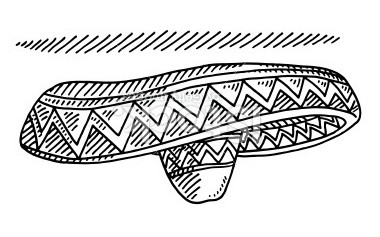
\includegraphics[width = 4cm]{mexicanhat.jpg} 
\end{subfigure}
\begin{subfigure}{0.49\textwidth}
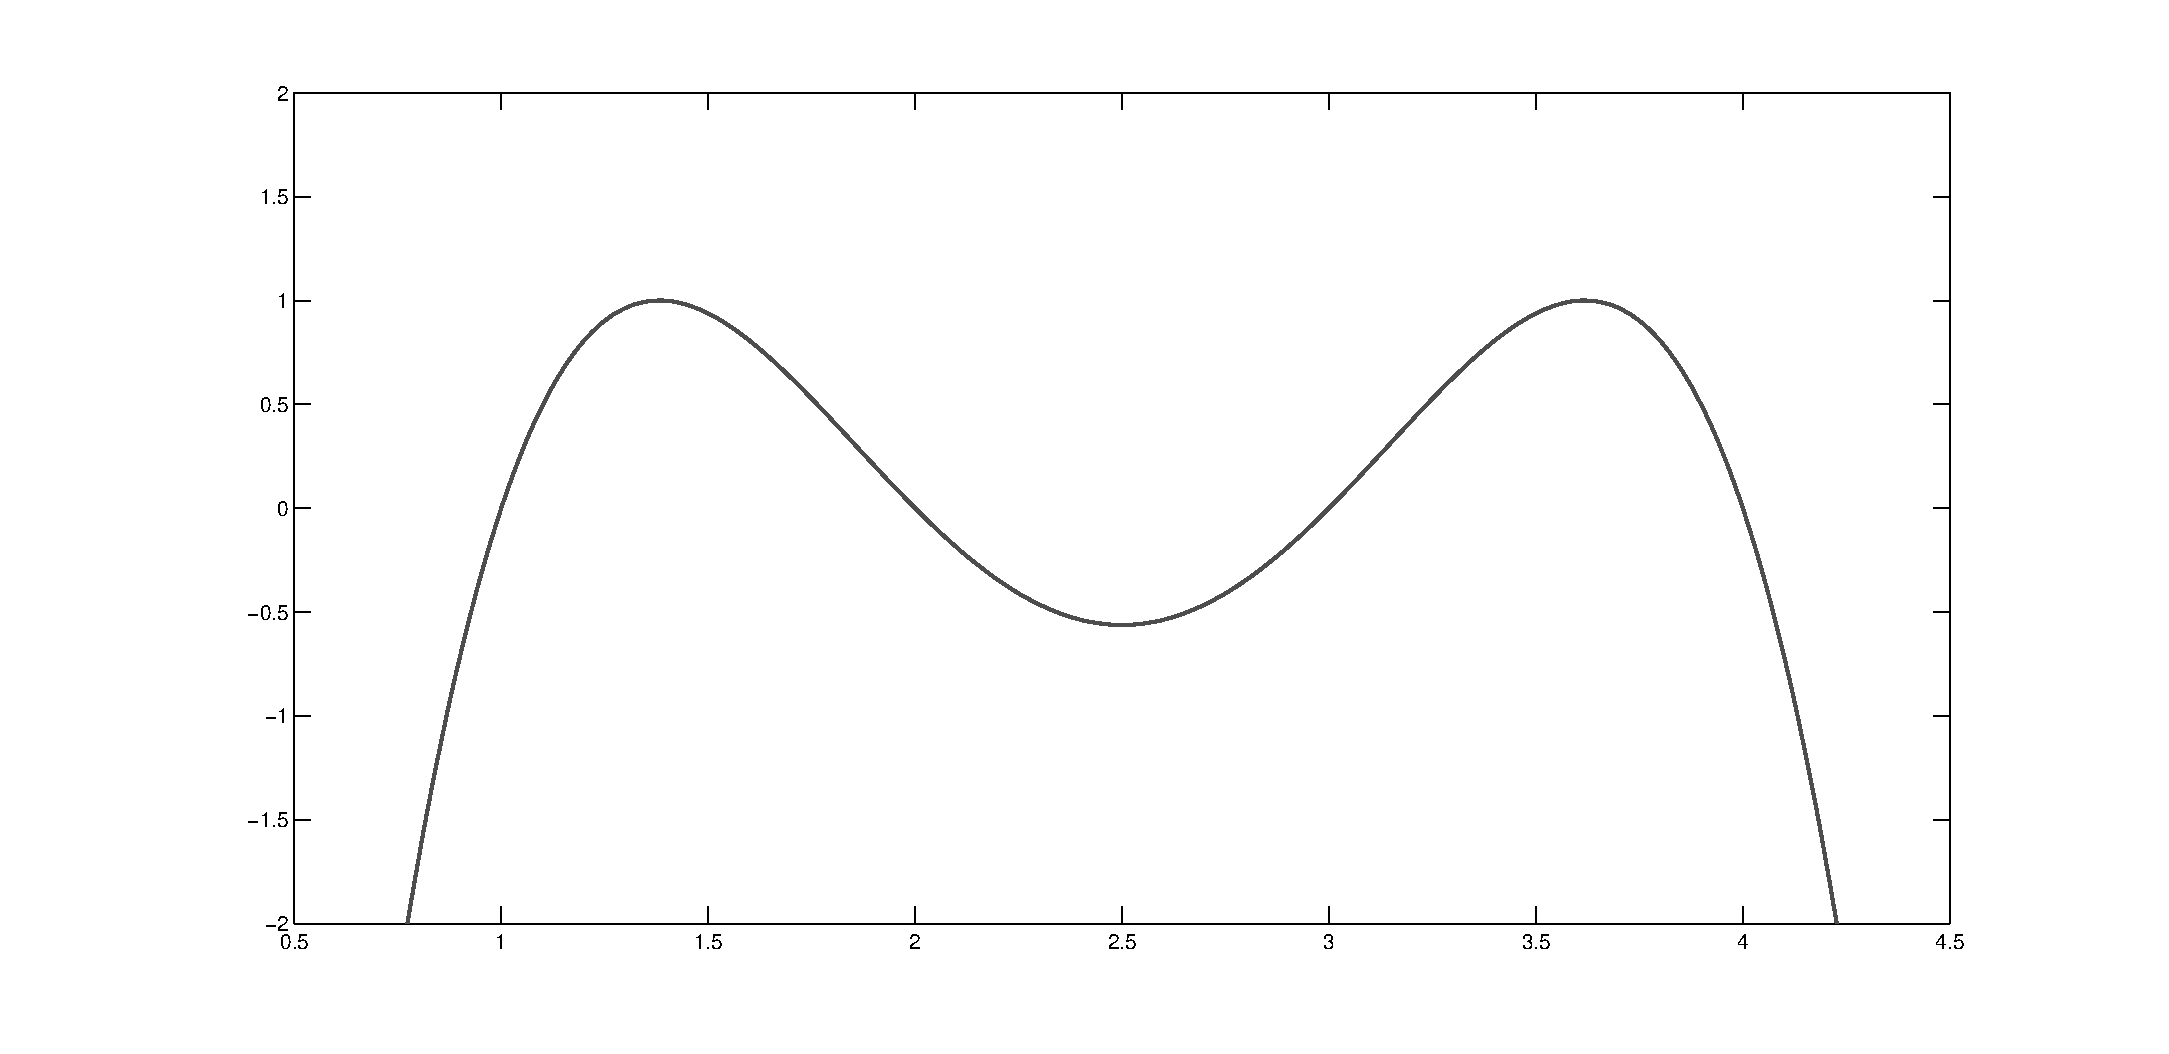
\includegraphics[width = 5cm]{mexicangraph.eps}
\end{subfigure}
\end{figure}
\begin{block}{}
If the weights are all positive, the system has a unique fixed point $r^{\star}$ in the domain.
\end{block}
\end{frame}

\begin{frame}
\frametitle{Influence of the parameter $k$}
\framesubtitle{Limitations}
\begin{block}{Domain for $k$}
\begin{itemize}
\item The greater the $k$, the more inconsistent judges will be penalized
\item The weights must be positive
$$k\in \mathcal{K} = \{k\in \mathcal{R}_{\geq 0} | 1 - k \begin{pmatrix} div_1 \\ div_2 \\ \vdots \\ div_n \end{pmatrix} >0 \: \forall r \in \mathcal{H} \}$$
\item In some cases, we would like to choose the highest $k$ possible
\end{itemize}
\end{block}

\end{frame}

\begin{frame}
\frametitle{Influence of the parameter $k$}
\framesubtitle{Modified method}
\begin{block}{Non-fixed $k$}
\begin{itemize}
\item Use of a sequence $k^t$
\item $k^t$ is such that at each iteration the weights are non-negative
$$ k^t : \min_i w_i^t = 0$$
%\item The sequence converges in general
\end{itemize}
\end{block}
\begin{block}{Shortcoming of the method}
\begin{itemize}
\item The greatest belief divergence limits the highest value of $k$.
\item Some cheaters with high belief divergence could shield other more subtle cheaters
\end{itemize}
\end{block}
\end{frame}

